\problemset{Статистический анализ}
\problemset{Индивидуальное домашнее задание №2}

\renewcommand*{\proofname}{Решение}

В результате эксперимента получены данные, приведенные в таблицах 1 и 2.

\textbf{Таблица 1.}

\begin{tabular}{|l|l|l|l|l|l|l|l|l|l|l|l|l|l|l|l|l|l|l|l|l|l|l|l|l|l|l|l|l|l|l|l|l|l|l|l|l|l|l|l|l|l|l|l|l|l|l|l|l|l|}
	\hline
	0&1&1&1&1&0&0&0&2&0&1&0&0&1&1&1&2&0&0&0&0&4&0&1&0\\ \hline 0&0&0&0&0&1&1&1&2&3&1&0&1&0&0&2&0&0&0&1&1&1&0&1&2\\
	\hline
\end{tabular}
\\ 

\textbf{Таблица 2.}

\begin{tabular}{|l|l|l|l|l|}
	\hline
	$\alpha_1=0.10$ & $a = 0.00$ & $b = 1.37$ & $\lambda_0=0.70$ & $\lambda_1=1.40$ \\
	\hline
\end{tabular}

%% Задание 1: условие
\begin{problem}
	Построить вариационный ряд, эмпирическую функцию распределения и гистограмму частот.
\end{problem}

%% Задание 1: решение
\begin{proof}
	$ $
		
	Вариационный ряд:\\
	0 0 0 0 0 0 0 0 0 0 0 0 0 0 0 0 0 0 0 0 0 0 0 0 0 1 1 1 1 1 1 1 1 1 1 1 1 1 1 1 1 1 1 2 2 2 2 2 3 4\\ 
	Построим таблицу частот для выборки.\\
	
	\textbf{Таблица 3.}
		
	\begin{tabular}{|c|c|c|c|c|c|}
		\hline
		$x_j$&0&1&2&3&4\\ \hline
		$m_j$&25&18&5&1&1\\ \hline
		$p_j^*$&\frc12&\frc9{25}&\frc1{10}&\frc1{50}&\frc1{50} \\
		\hline
	\end{tabular}
	\\
	
	Построим эмпирическую функцию распределения по полученным данным:\\
	 $F(x)=\left\{ 
	\begin{gathered} 
		0, x \leqslant 0 \hfill \\  
		0.5, 0 < x \leqslant 1 \hfill \\
		0.86, 1 < x \leqslant 2 \hfill \\
		0.96, 2 < x \leqslant 3 \hfill \\
		0.98, 3 < x \leqslant 4 \hfill \\
		1, x > 4 \hfill \\
	\end{gathered}
	\right.$\\ \\
	График представлен на рис. 1:\\ 
	\begin{figure}[h]
		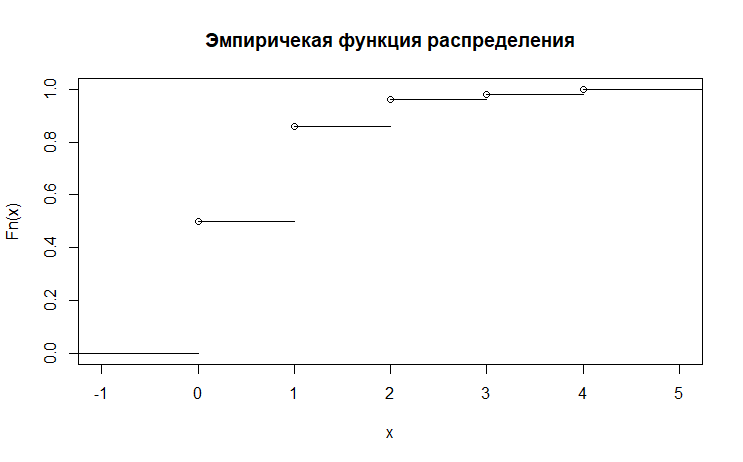
\includegraphics[scale=0.7]{Emp.png}
		\caption{Эмпирическая функция распределения}
	\end{figure}\\
	Гистограмма частот представлена на рис. 2:\\ 
	\begin{figure}[h]
		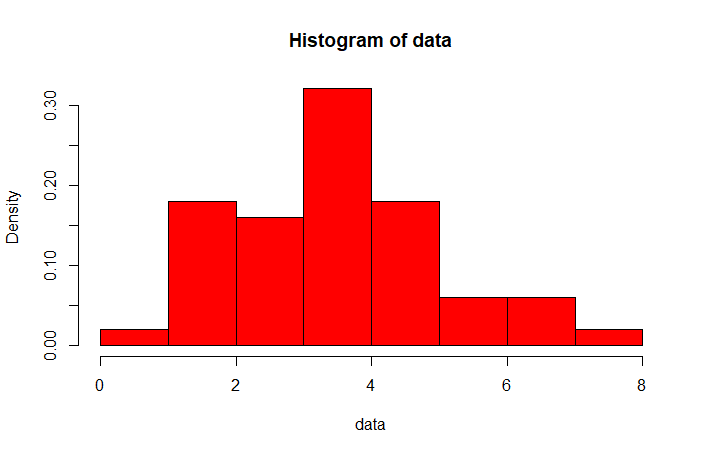
\includegraphics[scale=0.7]{Hist.png}
		\caption{Гистограмма частот}
	\end{figure}\\
	
\end{proof}

%\newpage
%% Задание 2: условие
\begin{problem}
	Вычислить выборочные аналоги следующих характеристик:
	\begin{itemize}
		\item математического ожидания
		\item дисперсии
		\item медианы
		\item ассиметрии
		\item эксцесса
		\item вероятности $P(X\in[a, b])$
	\end{itemize}
\end{problem}

%% Задание 2: решение
\begin{proof}
	$ $	
	\begin{itemize}
	\item Математическое ожидание:
		\begin{equation}	
		\bar x_{\text{в}} = \cfrac1n 		\sum^{n}_{i=1}x_im_i=\cfrac1{50}\cdot(18+10+7)=\cfrac{35}{50}=0.7
		\end{equation}
	\item Дисперсия:
	\begin{equation}	
		D_{\text{в}} = \bar{x^2}-\bar{x}^2=\cfrac1n\sum(x_i-\bar{x})^2=\cfrac1{50}\cdot(18+20+9+16)-0.49=\cfrac{63}{50}-0.49=1.26-0.49=0.77
	\end{equation}
	\item Медиана:
	\begin{equation}
		Me = \frc12
	\end{equation}	
	\item Ассиметрия:
	\begin{equation}
		As = \cfrac{\mu_3^*}{\sigma^3} = 1.509608
	\end{equation}
	\item Эксцесс:
	\begin{equation}
		Ex = \cfrac{\mu_4^*}{\sigma^4}-3 = 2.633496
	\end{equation}
	\item Вероятность:
	\begin{equation}
		P(x \in [a, b]) = P(x \in [0.00, 1.37]) = F(1.37) - F(0.00) = 0.86 
	\end{equation}
	\end{itemize}			
\end{proof}

\newpage
%% Задание 3: условие
\begin{problem}
	В предположении, что исходные наблюдения являются выборкой из распределения Пуассона, построить оценку максимального правдоподобия параметра $\lambda$, а также оценку $\lambda$ по методу моментов. Найти смещение оценок 	
\end{problem}

%% Задание 3: решение
\begin{proof}
	$ $ 
	
	Распределение Пуассона:
	$P_{\lambda} = (x = k) = \cfrac{\lambda^k}{k!}\cdot \exp(-\lambda)$
	\begin{itemize}
		\item Метод максимального правдоподобия
		\begin{multline}
			l(x, \lambda) =  \cfrac{\lambda^{\sum\limits^n_1x_i}\cdot \exp (-\lambda n)}{\prod\limits_1^n x_i!}\Rightarrow ll(\bar{x}, \lambda) = \sum\limits_1^nx_iln\lambda-n\lambda-\sum\limits_1^nlnx_i!\Rightarrow \cfrac{\partial ll(\bar x, \lambda)}{\partial \lambda} = \cfrac1{\lambda}\sum\limits_1^nx_i-n=0\Rightarrow \\ \Rightarrow \hat{\lambda}= \cfrac{1}{n}\sum\limits_1^nx_i=\bar{x_{\text{в}}}=0.7
		\end{multline}
		\item Метод моментов
		\begin{align}
			&P(x, \theta) \\
			&M_1^* = \bar{x_{\text{в}}}; \mathbb{E}X = \bar{x_{\text{в}}}; \\
			&\mathbb{E}X = \int_{\mathbb{R}}xp(x, \theta)dx = \varphi(\theta) \\
			&M_1 = \mathbb{E}X=\lambda; M_1^* = \bar{x_{\text{в}}} \Rightarrow \underline{\hat{\lambda} = \bar{x_{\text{в}}} = 0.7}
		\end{align}
	\end{itemize}
	Чтобы найти смещение оценки, найдем:
	\begin{equation}
		\mathbb{E}\hat{\lambda}=\cfrac1n\sum\limits_1^n\mathbb{E}x_i=\cfrac{n\lambda}n=\lambda\Rightarrow\text{оценки несмещенные}
	\end{equation}
\end{proof}

%\newpage
%% Задание 4: условие
\begin{problem}
	Построить асимптотический доверительный интервал уровня значимости $\alpha_1$ для параметра $\lambda$ на базе оценки максимального правдоподобия.	
\end{problem}

%% Задание 4: решение
\begin{proof}
	\begin{align}
		&\hat{\lambda}=\bar{x_{\text{в}}}=0.7; \alpha_1=0.10; \gamma=1-\alpha_1=0.90; \\
		&\cfrac{\sqrt{n}(\bar{x}-\lambda)}{\sqrt{\lambda}}\underset{n\to\infty}{\longrightarrow}N(0,1) \\
		&t_\gamma: \phi(t_\gamma)=1-\cfrac{\alpha_1}2\Rightarrow t_\gamma=1.645 \\
		&P(-t_\gamma \leqslant \cfrac{\sqrt{n}(\bar{x_\text{в}}-\lambda)}{\sqrt{\lambda}} \leqslant t_\gamma)\longrightarrow 1-\alpha \\
	    &n(\bar{x_\text{в}}-\lambda)^2=t_\gamma^2\lambda \\
		&\lambda^2-2\lambda(\bar{x_\text{в}}+\cfrac{t_\gamma^2}{2n})+\bar{x_\text{в}}=0 \\
		&D = \cfrac{t_\gamma^2}{n}(\bar{x_\text{в}}+\cfrac{t_\gamma^2}{4n}) \\
		&\lambda_{1,2}=\bar{x_\text{в}}+\cfrac{t_\gamma^2}{2n}\pm t_\gamma\sqrt{\cfrac1n(\bar{x_\text{в}}+\cfrac{t_\gamma^2}{4n})}=0.7+0.027\pm0.1965\Rightarrow [0.5305; 0.9235]
	\end{align}	
\end{proof}


%\newpage
%% Задание 5: условие
\begin{problem}
	Используя гистограмму частот, построить критерий значимости $\chi^2$ проверки простой гипотезы согласия с распределением Пуассона с параметром $\lambda_0$. Проверить гипотезу на уровне значимости $\alpha_1$. Вычислить наибольшее значение уровня значимости, на котором еще нет оснований отвергнуть данную гипотезу. 
\end{problem}

%% Задание 5: решение
\begin{proof}
	\begin{align}
		&\hat{\lambda_0}=0.70; \alpha_1=0.10; \\
		&m_i-\text{эмпирические частоты}; \\
		&m_i^{'}-\text{выравнивающие частоты}; m_i^{'}=n\cdot p_i \\
		&\text{Простая гипотеза } H_0 \text{ имеет вид:} \\
		&H_0:p(x)=\cfrac{\lambda_0^x}{x!}\exp(-\lambda_0) \\
		&\text{Тогда искомая вероятность примет вид:} \\
		&p_k=P(X=k)=\cfrac{0.7^k}{k!}\exp(-0.7) \\
	\end{align}	
	Построим таблицу оценки методом $\chi^2$.
	
	\textbf{Таблица 4.}
	
	\begin{tabular}{|c|c|c|c|c|c|c|}
		\hline
		$x_i$ & 0 & 1 & 2 & 3 & 4 & $\sum$ \\ \hline 
		$m_i$ & 25 & 18 & 5 & 1 & 1 & 50 \\ \hline 
		$p_i$ & 0.497 & 0.348 & 0.122 & 0.029 & 0.005 & 1 \\ \hline 
		$m_i^{'}$ & 25 & 17 & 6 & 1 & 1 & 50 \\ \hline 
		$m_i-m_i^{'}$ & 0 & 1 & -1 & 0 & 0 & 0 \\ \hline 
		$\cfrac{(m_i-m_i^{'})^2}{m_i^{'}}$ & 0 & $\cfrac1{17}=0.059$ & $\cfrac1{6}=0.167$ & 0 & 0 & $\chi^2_{\text{набл}}$ \\
		\hline
	\end{tabular}
	\\
	
	Итого
	\begin{align}
		&\chi^2_{\text{набл}}=\sum\limits_1^k\cfrac{(m_i-m_i^{'})^2}{m_i^{'}}=0.226 \\ 
		&l=k-r-1=5-1-1=3 \\
		&\chi^2_{\text{кр}}=\chi^2_{\alpha;l} = \chi^2_3 \text{ на уровне значимости 0.1 = 6.251} \\
	\end{align}
	$\chi^2_{\text{набл}} < \chi^2_{\text{кр}}\Rightarrow$ гипотеза $H_0$ принимается, выборка принадлежит распределению Пуассона.\\
	Наибольшее значение уровня значимости, при котором еще нет оснований отвернуть данную гипотезу = $0.8914$
	
\end{proof}


%% Задание 6: условие
\begin{problem}
	Построить критерий значимости $\chi^2$ проверки сложной гипотезы согласия с распределением Пуассона. Проверить гипотезу на уровне значимости $\alpha_1$. Вычислить наибольшее значение уровня значимости, на котором еще нет оснований отвергнуть данную гипотезу. 
\end{problem}

%% Задание 6: решение
\begin{proof}
	$ $
	
	Сложная гипотеза $H_0$ имеет вид:
	\begin{align}
		H_0: x_1,...,x_n \sim P_{ois}(\lambda) \\
		\sum\limits_1^k\cfrac{(m_i-np_i(\lambda))^2}{np_i(\lambda)}\longrightarrow\chi^2_{k-r-1}
	\end{align}	

	Метод минимизации хи-квадрат:
	\begin{equation}
		\underset{\lambda}{argmin}\sum\limits_1^r\cfrac{(m_i-np_i(\lambda))^2}{np_i(\lambda)}
	\end{equation}
	
	Задача реализована в R следующим скриптом:
	\begin{align}
		&P <- function(a)\{ \\
		&p <- 0\\
		&p[1] <- ppois(0, a)\\
		&p[2] <- ppois(1, a) - sum(p)\\
		&p[3] <- ppois(2, a) - sum(p)\\
		&p[4] <- ppois(3, a) - sum(p)\\
		&p[5] <- 1-sum(p)\\
		&p\}\\
		&X2 <- function(a)\{g <- n\cdot P(a); f <- (nu-g)^2/g; sum(f)\} \\
		&nu <- c(25, 17, 6, 1, 1) \\
		&XM <- nlm(X2, 0.70)\\
	\end{align}
	
	В результате вычислений получим, что $\chi^2_{\text{набл}}=1.5265<\chi^2_{\text{крит}}=4.6$ 
	Таким образом, гипотеза принимается. Наибольшее значение уровня значимости, при котором еще нет оснований отвернуть данную гипотезу = $0.74$	
\end{proof}


%% Задание 7: условие
\begin{problem}
	Построить наиболее мощный критерий проверки простой гипотезы пуассоновости с параметром $\lambda=\lambda_0=0.70$ при альтернативе пуассоновости с параметром $\lambda=\lambda_1=1.40$. Проверить гипотезу на уровне значимости $\alpha_1$. Что получится, если поменять местами основную и альтернативную гипотезы?
\end{problem}

%% Задание 7: решение
\begin{proof}
	$ $
	
	Сформулируем гипотезы. \\
	$H_0:\lambda=\lambda_0=0.70 \\ H_1:\lambda=\lambda_1=1.40$ \\
	По лемме Неймана-Пирсона: \\
		
	$\phi(\bar x)=\left\{
	\begin{gathered}
		0, \text{if } l(\bar x, \lambda_0, \lambda_1)<C \hfill \\
		p, \text{if } l(\bar x, \lambda_0, \lambda_1)=C \hfill \\
		1, \text{if } l(\bar x, \lambda_0, \lambda_1)>C \hfill \\ 
	\end{gathered}
	\right.$
	
	\begin{align}
		& l(\bar x, 0.7, 1.4)=\cfrac{L(\bar x, 1.4)}{L(\bar x, 0.7)}=2^{\sum x_i}\cdot \exp(n*(\lambda_0-\lambda_1))=2^{\sum x_i}\cdot \exp(-0.7n) \\
		& ll(\bar x, \lambda_0, \lambda_1)=-\sum x_i\cdot ln2-0.7n<lnC \\ 
		& \sum x_i > \cfrac{-lnC-0.7n}{ln2} \\
		& \hat{C}=\cfrac{-lnC-0.7n}{ln2} \\
	\end{align}
	Критерий принимает вид: \\
	
	$\phi(\bar x)=\left\{
	\begin{gathered}
		0, \text{if } \sum x_i>\hat{C} \hfill \\
		p, \text{if } \sum x_i=\hat{C} \hfill \\
		1, \text{if } \sum x_i<\hat{C} \hfill \\ 
	\end{gathered}
	\right.$	\\
	
	Вычислим $\hat{C}$ и $p$ из уравнения:		
	\begin{align}
		& P_{\lambda_0}(l(\bar x, \lambda_0, \lambda_1)>C)+p\cdot P_{\lambda_0}(l(\bar x, \lambda_0, \lambda_1)=C)= \\
		& = P_{\lambda_0}(\sum\limits_1^nx_i>\hat{C})+p\cdot P_{\lambda_0}(\sum\limits_1^nx_i=\hat{C})=\alpha_1=0.1 \\
		& x_i \rightarrow P_{ois}(\lambda_0) \\
		& \sum x_i \rightarrow P_{ois}(n\lambda_0) \\
	\end{align} 
	Подбором среди целых чисел можно найти такое наибольшее $\hat{C}$ и $\alpha_0$, что
	\begin{align}
		& \alpha_0=P_{\lambda_0}(\sum\limits_1^nx_i>\hat{C})=1-P_{n\lambda_0}(\hat{C})-p_{n\lambda_0}(\hat{C})<\alpha_1 \\
		& p=\cfrac{\alpha_1-\alpha_0}{P_{\lambda_0}(\sum\limits_1^nx_i=A)}=\cfrac{\alpha_1-\alpha_0}{p_{n\lambda_0}(A)} \\
	\end{align}
	В результате расчета получим: $\alpha_0=0.09867$; $\hat{C}=41$; $p=0.03499$
	\begin{equation}
		\sum\limits_1^nx_i=35
	\end{equation}
	\begin{equation}
		35<41\Rightarrow\text{ Таким образом, принимаем гипотезу} H_0 
	\end{equation}

	Теперь поменяем местами основную и альтернативную гипотезы.	\\
	
	$H_0:\lambda=\lambda_1=1.40$ 
	
	$H_1:\lambda=\lambda_0=0.70$ 
	\begin{align}
		& l(\bar x, 1.4, 0.7)=\cfrac{L(\bar x, 0.7)}{L(\bar x, 1.4)}=(\frac12)^{\sum x_i}\cdot \exp(n*(\lambda_1-\lambda_0))=(\frac12)^{\sum x_i}\cdot \exp(0.7n) \\
		& ll(\bar x, \lambda_0, \lambda_1)=-\sum x_i\cdot ln(\frac12)+0.7n<lnC \\ 
		& \sum x_i < \cfrac{lnC-0.7n}{ln(\frac12)} \\
		& \hat{C}=\cfrac{lnC-0.7n}{ln(\frac12)} \\
	\end{align}
	Тогда критерий примет вид: \\
	
	$\phi(\bar x)=\left\{
	\begin{gathered}
		0, \text{if } \sum x_i<\hat{C} \hfill \\
		p, \text{if } \sum x_i=\hat{C} \hfill \\
		1, \text{if } \sum x_i>\hat{C} \hfill \\ 
	\end{gathered}
	\right.$	\\
	
	Вычислим $\hat{C}$ и $p$ из уравнения:		
	\begin{align}
		& P_{\lambda_1}(\sum\limits_1^nx_i>\hat{C})+p\cdot P_{\lambda_1}(\sum\limits_1^nx_i=\hat{C})=\alpha_1=0.1 \\
		& p=\cfrac{\alpha_1-\alpha_0}{P_{\lambda_1}(\sum\limits_1^nx_i=A)}=\cfrac{\alpha_1-\alpha_0}{p_{n\lambda_1}(A)} \\
	\end{align}
	В результате расчета получим: $\alpha_0=0.081593$; $\hat{C}=58$; $p=1.049973$
	\begin{equation}
		\sum\limits_1^nx_i=35
	\end{equation}
	\begin{equation}
		35<58\Rightarrow\text{ Таким образом, отвергаем гипотезу} H_0 
	\end{equation}
	
	При замене основной и альтернативной гипотезы меняется также гипотеза, которая принимается. Но так как изменение происходит со сменой гипотез местами, решение не меняется.
\end{proof}


%% Задание 8: условие
\begin{problem}
	В пунктах (c) - (f) заменить семейство распределений Пуассона на семейство геометрических распределений
\end{problem}

%% Задание 8: решение
\begin{proof}
	$ $
	\begin{equation}
		P_{\lambda}(X=k)=\cfrac{\lambda^k}{(\lambda+1)^{k+1}}, k = 0, 1, ...
	\end{equation}
\end{proof}

%% Задание 3: условие
\begin{problem}
	В предположении, что исходные наблюдения являются выборкой из геометрического распределения, построить оценку максимального правдоподобия параметра $\lambda$, а также оценку $\lambda$ по методу моментов. Найти смещение оценок 	
\end{problem}

%% Задание 3: решение
\begin{proof}
	$ $ 
	
	Плотность геометрического распределения имеет вид:
	\begin{equation}
		P_{\lambda}(X=k)=\cfrac{\lambda^k}{(\lambda+1)^{k+1}}
	\end{equation}
	
	\begin{itemize}
		\item Метод максимального правдоподобия
		\begin{align}
			& l(\bar{x}, \lambda)=\prod\limits_1^n\cfrac{\lambda^{x_i}}{(\lambda+1)^{x_i+1}}=\cfrac{\lambda^{\sum\limits_1^nx_i}}{(\lambda+1)^{\sum\limits_1^nx_i+n}} \\
			& ll(\bar{x}, \lambda)=ln\lambda\cdot \sum\limits_1^nx_i-ln(\lambda+1)\sum\limits_1^nx_i-nln(\lambda+1) \\
			& \cfrac{\partial ll}{\partial \lambda}=\cfrac{1}{\lambda}\sum\limits_1^nx_i-\cfrac{1}{\lambda+1}\sum\limits_1^nx_i-\cfrac{n}{\lambda+1} \\
			& \cfrac{\partial ll}{\partial \lambda}=0\rightarrow\hat{\lambda}=\cfrac{1}{n}\sum\limits_1^nx_i=\bar{x}=0.7
		\end{align}
		\item Метод моментов
		\begin{align}
			& M_1 = \mathbb{X}=\lambda \\
			& M_1^*=\hat{X} \\
			& \hat{\lambda}=\bar{X} 
		\end{align}
	\end{itemize}
	Чтобы найти смещение оценки, найдем:
	\begin{equation}
		\mathbb{E}\hat{\lambda}=\mathbb{E}\hat{X}=\cfrac1n\sum\limits_1^n\mathbb{E}(x_i)=\cfrac{n\lambda}n=\lambda\Rightarrow\text{оценки несмещенные}
	\end{equation}
\end{proof}

%\newpage
%% Задание 4: условие
\begin{problem}
	Построить асимптотический доверительный интервал уровня значимости $\alpha_1=0.10$ для параметра $\lambda$ на базе оценки максимального правдоподобия.	
\end{problem}

%% Задание 4: решение
\begin{proof}
	\begin{align}
		& \cfrac{\partial^2ll}{\partial\lambda^2}=\cfrac{1}{\lambda^2}\sum\limits_1^nx_i+\cfrac{1}{(\lambda+1)^2}\sum\limits_1^nx_i+\cfrac{n}{(\lambda+1)^2} \\
		& \hat{I}=-\cfrac{\partial^2ll}{\partial\lambda^2}(\hat{\lambda})=-\cfrac{\partial^2ll}{\partial\lambda^2}(\hat{X})=n(\cfrac{1}{\bar{X}}-\cfrac{1}{\bar{X}+1})=42.017 \\
		& \sigma^2(\hat{\lambda})=\hat{I}^{-1}=0.024 \\
		& \sigma=\sqrt{\hat{I}^{-1}}=0.154 \\
		& \text{Доверительный интервал будет иметь вид} \\
		& [\hat{\lambda}-x_{\alpha}\sigma, \hat{\lambda}+x_{\alpha}\sigma] \\
		& x_{\alpha}=\phi^{-1}(1-\frac{\alpha_1}{2})=1.645 \\
		& \text{Получен доверительный интервал } [0.4467, 0.9534]
	\end{align}	
\end{proof}

%\newpage
%% Задание 5: условие
\begin{problem}
	Используя гистограмму частот, построить критерий значимости $\chi^2$ проверки простой гипотезы согласия с геометрическим распределением с параметром $\lambda_0=0.70$. Проверить гипотезу на уровне значимости $\alpha_1=0.10$. Вычислить наибольшее значение уровня значимости, на котором еще нет оснований отвергнуть данную гипотезу. 
\end{problem}

%% Задание 5: решение
\begin{proof}
	\begin{align}
		&H_0: X_1, ..., X_n \sim Geom\left(\cfrac{1}{0.7+1}\right)=Geom\left(\cfrac{1}{1.7}\right)
	\end{align}	
	Построим таблицу оценки методом $\chi^2$.
	\newpage	
	\textbf{Таблица 5.} \\
	
	\begin{tabular}{|c|c|c|c|c|c|c|}
		\hline
		$x_i$ & 0 & 1 & 2 & 3 & 4 & $\sum$ \\ \hline 
		$m_i$ & 25 & 18 & 5 & 1 & 1 & 50 \\ \hline 
		$p_i$ & 0.59 & 0.242 & 0.099 & 0.040 & 0.017 & 1 \\ \hline 
		$m_i^{'}$ & 29 & 12 & 5 & 2 & 2 & 50 \\ \hline 
		$m_i-m_i^{'}$ & -4 & 6 & 0 & -1 & -1 & 0 \\ \hline 
		$\cfrac{(m_i-m_i^{'})^2}{m_i^{'}}$ & $\cfrac{16}{29}=0.55$ & $\cfrac{36}{12}=3$ & 0 & $\cfrac12=0.5$ & $\cfrac12=0.5$ & $\chi^2_{\text{набл}}$ \\
		\hline
	\end{tabular}
	\\
	
	Итого
	\begin{align}
		&\chi^2_{\text{набл}}=\sum\limits_1^k\cfrac{(m_i-m_i^{'})^2}{m_i^{'}}=4.55 \\ 
		&l=k-r-1=5-1-1=3 \\
		&\chi^2_{\text{кр}}=\chi^2_{\alpha;l} = \chi^2_3 \text{ на уровне значимости 0.1 = 6.251} \\
	\end{align}
	$\chi^2_{\text{набл}} < \chi^2_{\text{кр}}\Rightarrow$ гипотеза $H_0$ принимается, выборка принадлежит геометрическому распределению. Наибольшее значение уровня значимости, при котором еще нет оснований отвернуть данную гипотезу = $0.79213$	
\end{proof}

%% Задание 6: условие
\begin{problem}
	Построить критерий значимости $\chi^2$ проверки сложной гипотезы согласия с геометрическим распределением. Проверить гипотезу на уровне значимости $\alpha_1=0.10$. Вычислить наибольшее значение уровня значимости, на котором еще нет оснований отвергнуть данную гипотезу. 
\end{problem}

%% Задание 6: решение
\begin{proof}
	$ $
	
	Сложная гипотеза $H_0$ имеет вид:
	\begin{align}
		H_0: X_1, ..., X_n \sim Geom\left(\cfrac{1}{1+\lambda}\right) \\
		\sum\limits_1^r\cfrac{(m_i-np_i(\lambda))^2}{np_i(\lambda)}\longrightarrow\chi^2_{k-r-1}
	\end{align}	
	
	Метод минимизации хи-квадрат:
	\begin{equation}
		\underset{\lambda}{argmin}\sum\limits_1^k\cfrac{(m_i-np_i(\lambda))^2}{np_i(\lambda)}
	\end{equation}
	
	Задача реализована в R следующим скриптом:
	\begin{align}
		&P <- function(a)\{ \\
		&p <- 0\\
		&p[1] <- pgeom(0, a)\\
		&p[2] <- pgeom(1, a) - sum(p)\\
		&p[3] <- pgeom(2, a) - sum(p)\\
		&p[4] <- pgeom(3, a) - sum(p)\\
		&p[5] <- 1-sum(p)\\
		&p\}\\
		&X2 <- function(a)\{g <- n\cdot P(a); f <- (nu-g)^2/g; sum(f)\} \\
		&nu <- c(25, 17, 6, 1, 1) \\
		&XM <- nlm(X2, 1/(1+0.70))\\
	\end{align}
	
	Получили оптимальную $\hat{\lambda}=\cfrac1{0.56559}-1=0.768$ \\
	
	Построим таблицу оценки методом $\chi^2$. 
		
	\textbf{Таблица 6.} \\
	
	\begin{tabular}{|c|c|c|c|c|c|c|}
		\hline
		$x_i$ & 0 & 1 & 2 & 3 & 4 & $\sum$ \\ \hline 
		$m_i$ & 25 & 18 & 5 & 1 & 1 & 50 \\ \hline 
		$p_i$ & 0.566 & 0.246 & 0.107 & 0.046 & 0.020 & 1 \\ \hline 
		$m_i^{'}$ & 28 & 13 & 6 & 2 & 1 & 50 \\ \hline 
		$m_i-m_i^{'}$ & -3 & 5 & -1 & -1 & 0 & 0 \\ \hline 
		$\cfrac{(m_i-m_i^{'})^2}{m_i^{'}}$ & $\cfrac{9}{28}=0.32$ & $\cfrac{25}{13}=1.92$ & $\cfrac{1}{6}=0.17$ & $\cfrac12=0.5$ & $0$ & $\chi^2_{\text{набл}}$ \\
		\hline
	\end{tabular} \\

	В результате вычислений получим, что $\chi^2_{\text{набл}}=2.91<\chi^2_{\text{крит}}=4.6$ 
	 
	Таким образом, гипотеза принимается. Наибольшее значение уровня значимости, при котором еще нет оснований отвернуть данную гипотезу = $0.572998$	
\end{proof}

\newpage


